%-*-coding: utf-8-*-

\chapter{Обзор предметной области}

\section{Постановка задачи}
\noindent Пусть есть некоторый язык со словарем $V$.\\
Пусть есть некоторая функция ошибки $L:\mathbb{R}^s \to \mathbb{R}$.\\
Пусть $D$~--- множество последовательностей над $V$, называемое датасетом задачи.\\
Задача построения векторного представления предложения, состоит в изобретении такой модели $M$, 
которая для любой последовательности слов $w \in V^n$ (любому предложению) сопоставляет
вектор $M(w) \in \mathbb{R}^s$ так, что суммарная ошибка $$\sum_{w \in D} L(M(w))$$ была как можно меньше.
Чем меньше эта ошибка, тем более качественна модель $M$.\\

\section{Решаемые задачи}
В данной работе будет предложена модель, качество которой будет оценено на задачах классификации эмоционального тона предложения и классификации вопросов.
\vspace{5mm}

\noindent \textbf{Задача классификации эмоционального тона предложения}\par
Задача классификации эмоционального тона предложения состоит в оценке эмоциональной характеристики предложения. Например, в данной работе будут рассмотрены датасеты, которые содержат обзоры фильмов. Предложенная модель должна будет предсказать, какому из пяти эмоциоанльных классов относится обзор:
\emph{очень негативный}, \emph{негативный}, \emph{нейтральный}, \emph{позитивный}, \emph{очень позитивный}.
\vspace{5mm}

\noindent \textbf{Задача классификации вопросов}\par
Задача классификации вопросов состоит в определении к какому типу принадлежит вопрос:
аббревиатура, сущность (животное, еда и т.д), описательный, личность, расположение, числовой.

Данные классы включают в себя более точные подклассы, на которых также будет проведена оценка модели.

\section{Вспомогательные понятия}

\subsection{Векторное представление слов}
Векторное представление слова (word embedding)\cite{Bengio03aneural}~--- параметризованное отображение слова на пространство большой размерности $\mathbb{R}^d$. 
Такое представление сохраняет семантические отношения между словами. 
Причем, похожим словам сопоставляются близкие по некоторой метрике вектора, 
а различным~--- удаленные друг от друга.

Векторное представление слов либо обучают <<с нуля>> вместе с основной моделью, либо берут за основу предобученные на достаточно большом корпусе текстовых данных. Наиболее крупные корпусы векторных представлений это word2vec\cite{DBLP:journals/corr/MikolovLS13, wor2vec}, а также GloVe\cite{pennington2014glove, glove}, которые также будут использоваться в данной работе.

\subsection{Дерево синтаксического разбора предложения}
Существует несколько способов построения дерева синтасксического разбора.
Это зависит от принципов построения и сущностей, которые поддерживает дерево зависимостей.
Так, например, существуют Stanford Dependencies\cite{standeps}, а также Universal Dependencies\cite{unideps}.
В данной работе будет использоваться преимущественно способ Probabilistic Context-Free Grammars\cite{pcfg}.

Данный способ задается грамматикой, по которой и разбирается предложение\cite{Klein03accurateunlexicalized}.
По языку строятся подкатегории фраз, например, такие как "noun phrase" (NP), "verb phrase" (VP) и т.д. 
Для них также строятся правила вывода грамматики, например, возможна следующая грамматика:
$$S \to NP VP$$
$$NN \to man | dog | \cdots$$

После чего предложение разбирается по этим правилам. 

\begin{figure}[h]
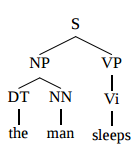
\includegraphics[scale=0.7]{pcfgs}
\caption{\textbf{Пример разбора предложения PCFG парсером}}
\label{fig:pcfgs}
\end{figure}

Данная граматика может быть неоднозначна, 
поэтому вывод происходит вероятностно~--- выбирается наиболее вероятное правило в данном контексте.

Вообще говоря, предложенная модель не зависит от способа построения дерева разбора и языка.

\section{Обзор существующих решений}

В данной главе будут приведены существующие решения для построения векторного представления предложения.

\subsection{Мешок слов}
Одним из первых подходов для анализа текстовых данных, 
является так называемый мешок слов (от англ. bag of words)[ссылка].
Данный подход не учитывает ни грамматические закономерности между словами, ни даже порядок слов.
Предложение рассматривается как мультисет слов.

Метод получил некоторые усовершенствования, такие как $NBoW$ (Neural Bag of Words), 
в котором рассматриваются не только предложение, но фразы в предложении из одного, двух и более слов[статья].

\subsection{Paragraph Vector}
Целью подхода Paragraph Vector является сопоставление вещественного вектора в $\mathbb{R}^d$ последовательности слов произвольной длины: предложению, абзацу или даже документу[статья].
Paragraph Vector учитывает семантический контекст текста на котором он получен.

Параметрами Paragraph Vector являются: вещественная матрица $W$~--- векторное представление слов словаря текстового корпуса, а также вещественная матрица $D$~--- векторное представление абзацев корпуса. Метод пытается предсказать следующее слово в абзаце, опираясь на векторное представление данного абзаца, а также слов из абзаца, смежных с предсказываемым словом, то есть находящихся в одном контексте с ним.

\begin{figure}[h]
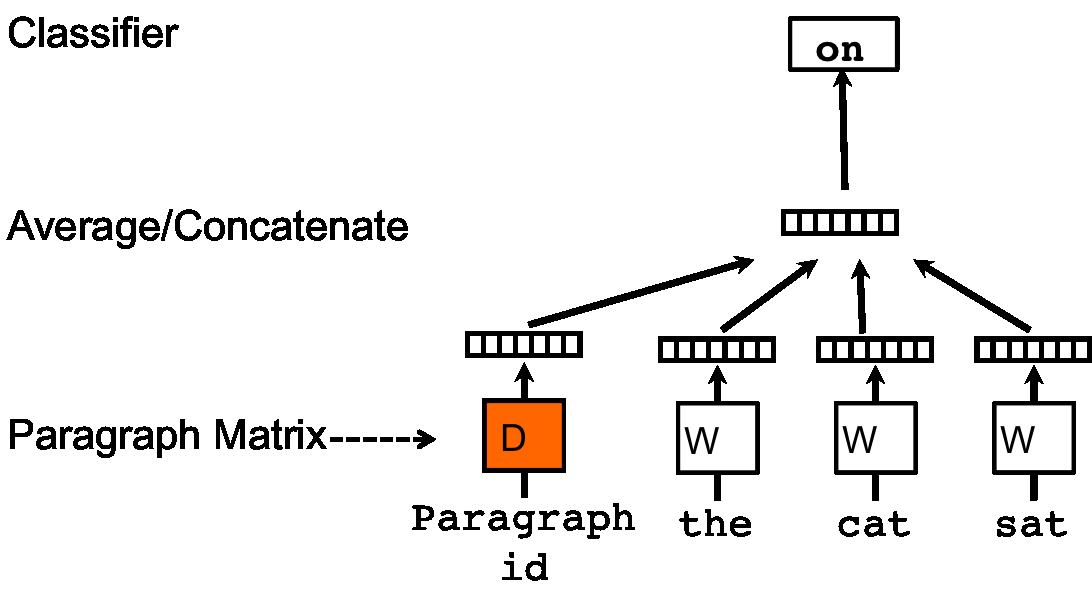
\includegraphics[scale=0.4]{par_vec}
\caption{\textbf{Paragraph Vector}}
\label{fig:par_vec}
\end{figure}

\subsection{Рекуррентная нейронная сеть}
Основным инструментом для обработки текстов являются так называемые \emph{рекуррентные нейронные сети}(РНС)[статьи].

Рекуррентные нейронные сети предназначены (РНС) для обработки последовательных данных, таких как звук и текст. В традиционных нейронных сетях все входы считаются независимыми друг от друга, но для многих задач это не так, и такой подход не учитывает много информации о структуре данных.

РНС принимает слова последовательности поочереди, сохраняя внутри себя контекст уже принятого текста. Рекуррентными они называются потому что выполняют одну и ту же задачу для каждого слова в тексте. Данная архитекутра достаточно хорошо отражает процесс восприятия информации человеком: после того как мы прочли начало предложение, в нашей голове уже сформировался некоторый контекст, и следующее слово обрабатывается нами с учетом уже прочитанной информации, а не воспринимается с чистого листа.

\begin{figure}[h]
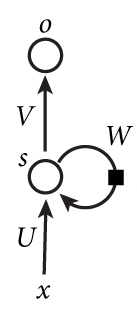
\includegraphics[scale=0.7]{rnn}
\caption{\textbf{РНС}}
\label{fig:rnn}
\end{figure}

\begin{figure}[h]
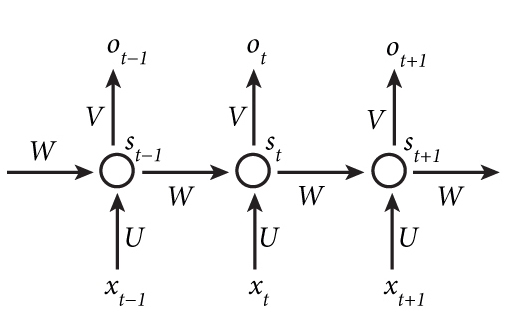
\includegraphics[scale=0.7]{rnn-unfold}
\caption{\textbf{РНС в развернутом виде}}
\label{fig:rnn-unfold}
\end{figure}

\noindent $U, W, V$~--- параметры РНС сети\\
$x_t$~--- вектор, соответствующий слову $t$ \\
$s_t$~--- информация о первых $t$ словах \\
$o_t$~--- выходной вектор

Хотя РНС является достаточно мощной моделью, у нее есть ряд недостатков, самый большой из которых~--- это так называемая <<проблема затухания градиента>>. Суть ее заключается в том, что РНС не может запоминать контекст в длинных последовательностях слов. Поэтому на смену РНС была изобретена другая архитектура РНС, под названием \emph{долгая краткосрочная память} (ДКП) (от англ. Long Short Term Memory или LSTM), которая решает эту проблему[статья].

\begin{figure}[h]
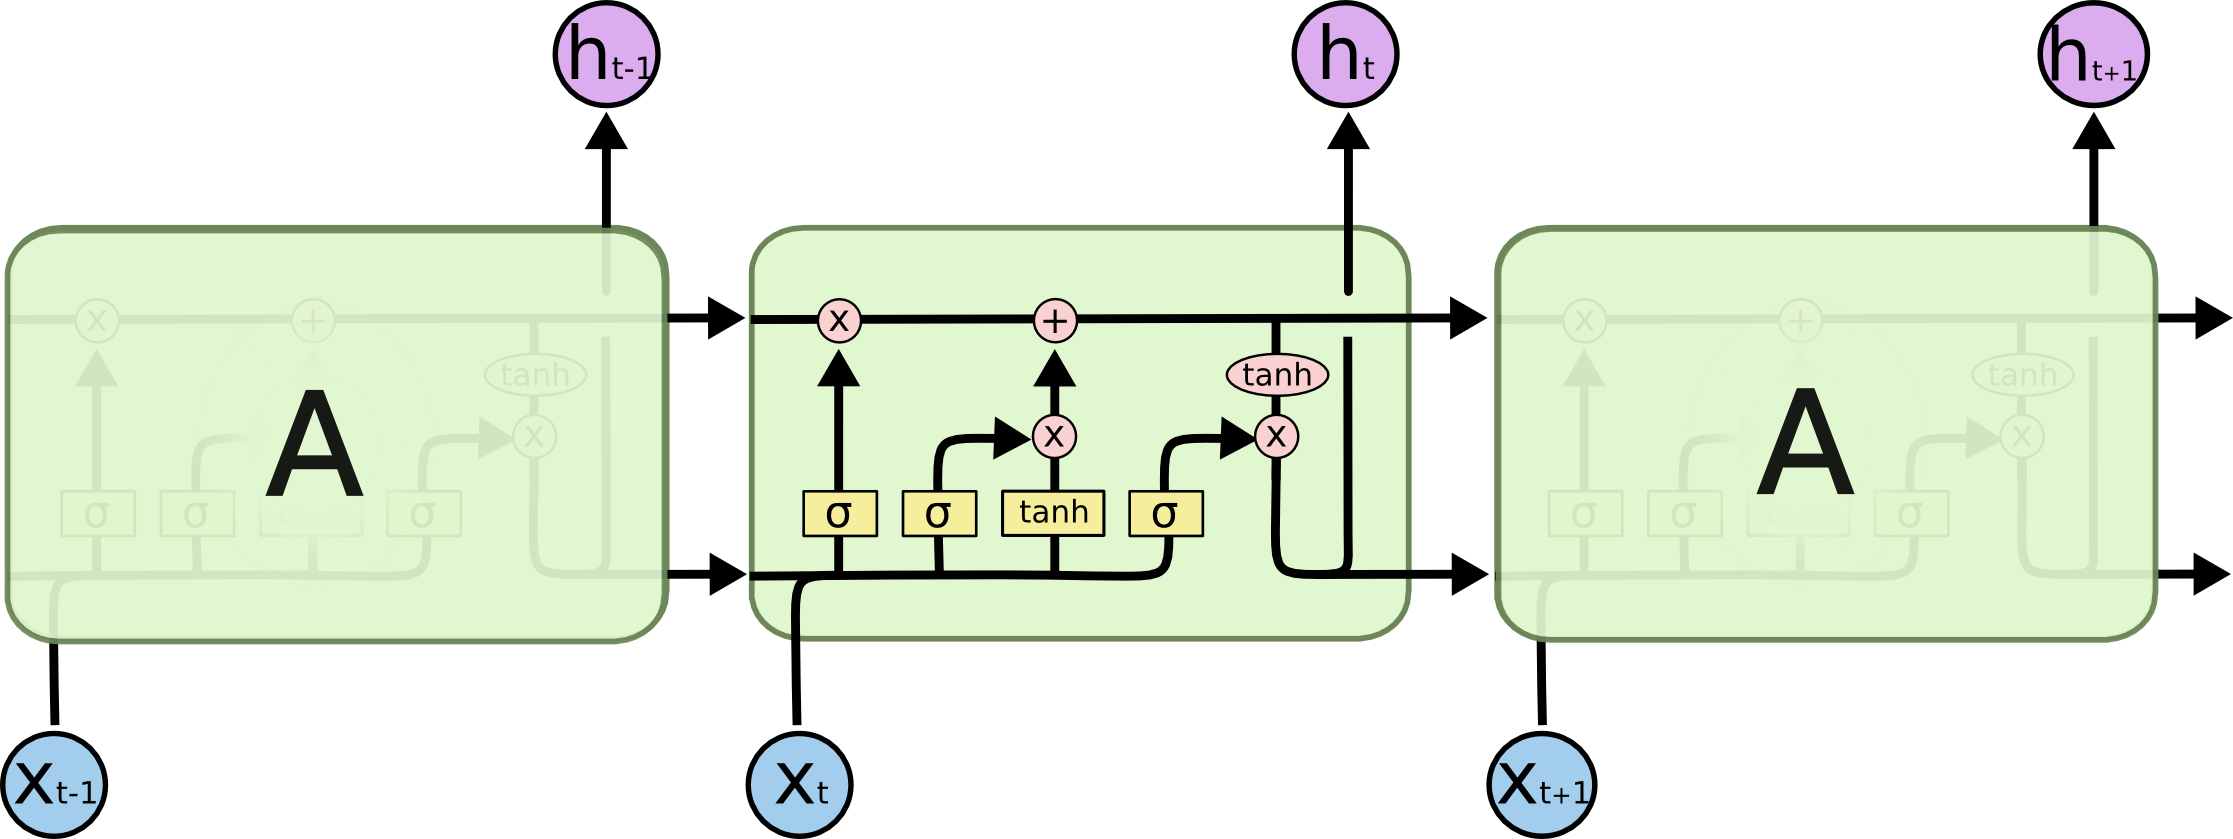
\includegraphics[scale=0.5]{lstm}
\caption{\textbf{Долгая краткосрочная память}}
\label{fig:lstm}
\end{figure}

Таким образом, на вход ДКП подается предложение, и используется последний выходной вектор как векторное представление для задачи sentiment modelling [статья].

\subsection{Сверточная нейронная сеть}
Сверточная нейронная сеть (СНС)~--- успешно показала себя в обработке и анализе изображений.[статья] Они работают подобно тому, как происходит распознавание образов в головной коре человека. СНС состоят из нескольких слоев, каждый из которых детектирует некоторые визуальные признаки изображения, такие как прямые линии, окружности. Признаки с предыдущего слоя используются для формирования более высокоуровневых визуальных признаков.

Преимуществом СНС является выделение локалных пространственных признаков [статья]. В контексте изображений это означает, что визуальные признаки локализуются сначала на неболших квадратах, а далее объединяются в большие фигуры.

Оказывается, данный плюс можно использовать и в задаче sentiment modelling, если рассмотреть слова предложения как вектора некоторой размерности. Тогда если в предложении $n$ слов, 
и размерность векторного представления слова $d$, получаем матрицу $n \times d$, 
которую можно трактовать как изображение и применить к нему сверточную нейронную сеть.[статья].

\begin{figure}[h]
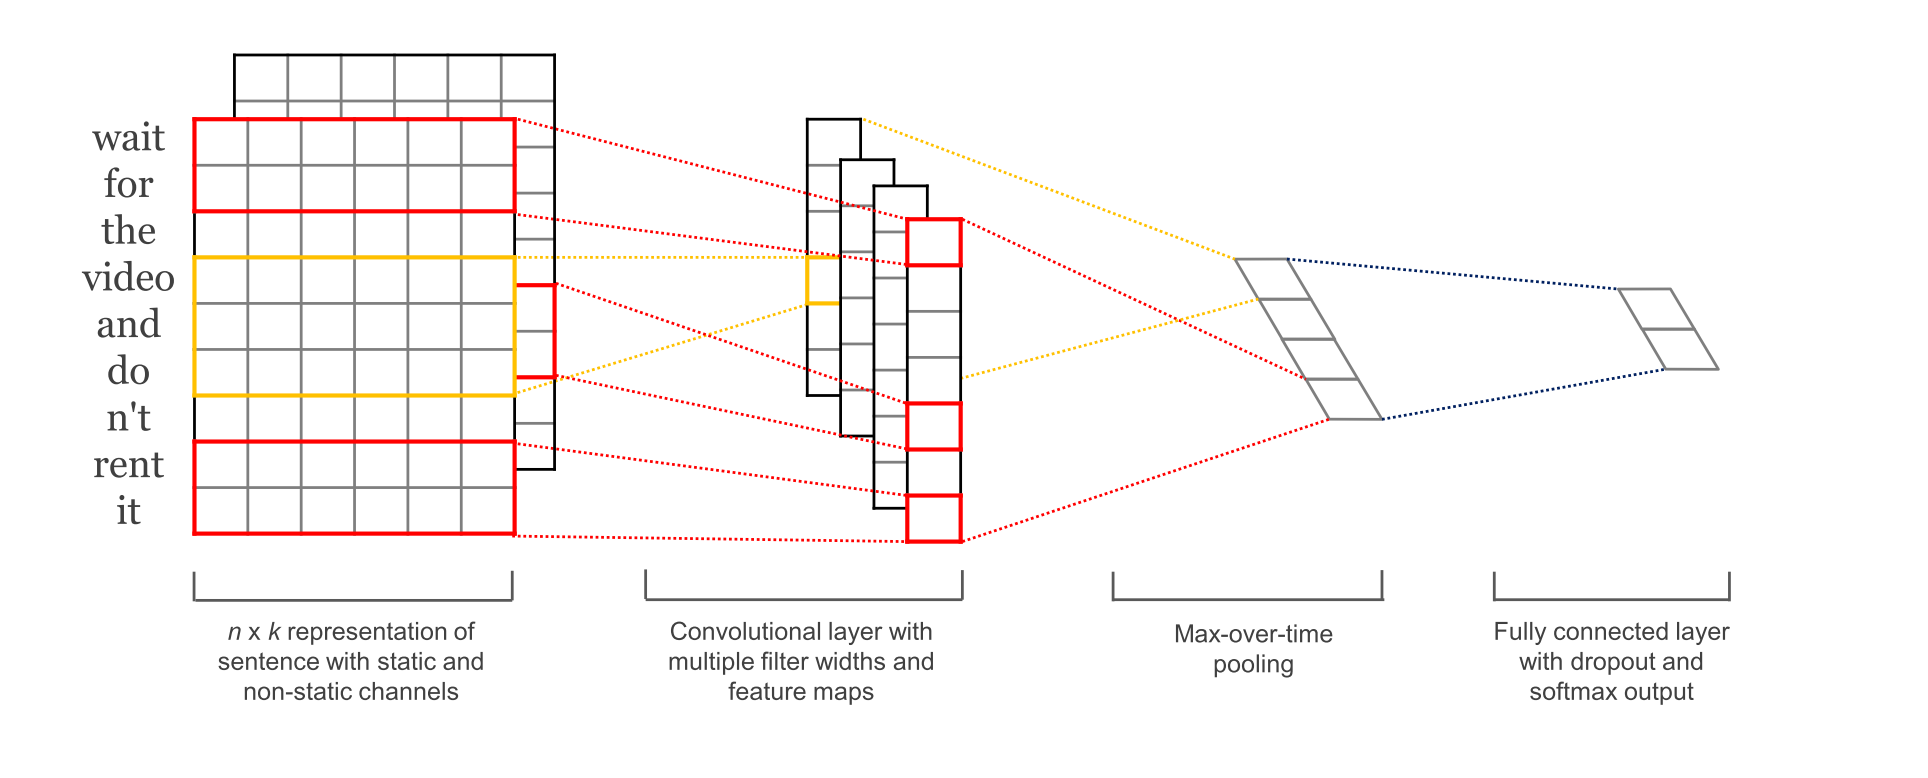
\includegraphics[scale=0.55]{cnn}
\caption{\textbf{СНС для предложения}}
\label{fig:cnn}
\end{figure}

\subsection{Рекуррентная тензорная нейронная сеть}
Еще одним важным подходом к решению задачи sentence modelling является использование 
дерева синтаксического разбора предложения. Вообще говоря, решения, использующие этот подход, предполагают, что у предложения уже построено дерево синтаксического разбора. Построение дерева является отдельной достаточно важной задачей NLP. На данный момент существуют алгоритмы, которые делают это построение с очень хорошей точностью[статьи]. 
С другой стороны, обычно для таких решений не столь важно точное построение дерева, то есть они не критичны к неточностям в дереве разбора.

Рекуррентная тензорная нейронная сеть (РТНС)~--- одно из решений, использующее дерево синтаксического разбора. Целью данного метода является сопостовление каждой вершине дерева разбора вектора в $R^d$, 
который и характеризует семантическое содержание фразы, соответствующей поддереву этой вершины.
Вектор для вершины $p$ вычисляется как $f(p)=g(f(c_1), f(c_2) \dots{} f(c_k))$, где $c_i$~--- непосредственные потомки вершины $p$, а $g$~--- некоторая функция. Вычисление происходит снизу-вверх, то
есть от листьев дерева к его корню. Для листьев $f(p)$ берутся произвольными и улучшаются в результате обучения в соответствии с поставленной задачей.
В качестве функции $g$ в оригинальной работе[статья] используется умножение на $n$-мерный тензор.

\begin{figure}[h]
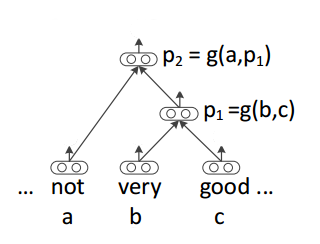
\includegraphics[scale=0.7]{rntn}
\caption{\textbf{Рекурсивная тензорная нейронная сеть}}
\label{fig:rntn}
\end{figure}
 
%\subsection{Численные оценки качества задачи классификации}

%Задача классификации формулируется следующим образом:

%Пусть $X$~--- множество объектов, $Y$~--- множество классов,
%существует отношение $y* : X \rightarrow Y$, заданное только для обучающей выборки.
%Необходимо построить такой алгоритм $a: X \rightarrow Y$, способный для произвольного
%$x \in X$ найти $y \in Y$.	

%\textbf{Точность}\\
%Точность (от англ. accuracy)~--- это один из самых простых способов оценить
%решение задачи классификации. Точность вычисляется следующим образом.

%$$Accuracy =\frac{P}{N}$$
%$P$~--- количество верно классифицированных объектов\\
%$N$~--- количество объектов в выборке

%\textbf{Кросс-энтропийная функция ошибки}\\